\subsection{Complexity}
Finally, below we have a plot outlining the computation times measured against $O(Nlog(N))$.
\begin{figure}[htb]
    \begin{center}
        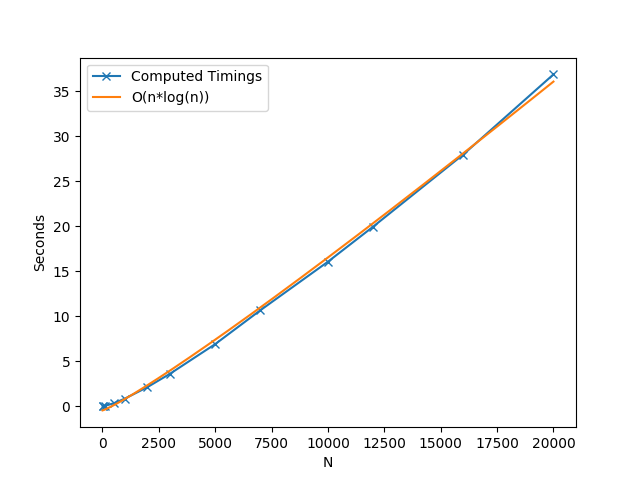
\includegraphics[width=8cm]{../images/nlogn.jpg}
        \caption{Time Complexity Plot}
    \end{center}
\end{figure}

We have then compared this method to the naive approach to see how much more effective it is as we increase the number of particles. As we can see, to begin with the naive approach has better computation time, but as the number of particles increases, the Barnes Hut algorithm shows its potential to calculate these things much more efficiently.
\begin{figure}[htb]
    \begin{center}
        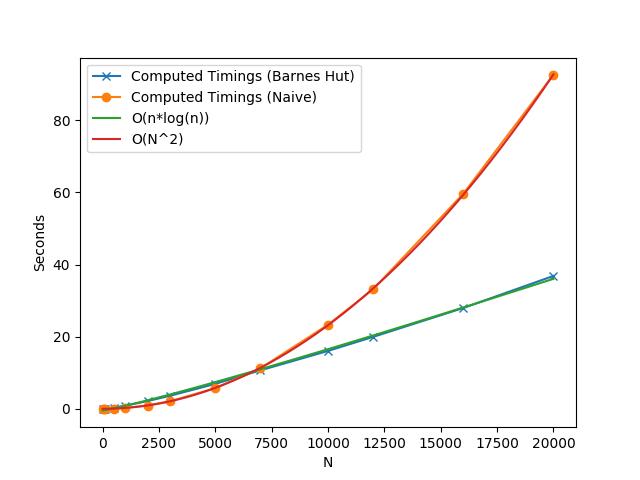
\includegraphics[width=8cm]{../images/complexity_compare.png}
        \caption{Time Complexity Plot}
    \end{center}
\end{figure}
\newpage
